\chapter{Lateral histograms}
This chapter treats of lateral histograms, which in our case simplify to row and column sums of the image. Although being very simple in principle, the lateral histograms show as a strong and robust method for EPOH and ECH detection. The largest part of its success, however, depends on the methods for estimating the period from the histograms. We present several such methods, perform experiments on them and compare them based on the experimental results.

\section{Lateral histograms applied to ionograms}
Lateral histograms are a little more general notion than we need in ionograms. We first provide the general definition and then we look for the more specialized one. We also observe a great simplification brought to this method by the nature of ionograms.

\subsection{Definition}
The general definition of lateral histograms is that ``the lateral histogram technique involves projecting an image on two or more axes by summing pixel intensities [\ldots] and using the resulting histograms to identify objects in the image.'' \citep{Davies2004} As can be seen, the title ``histograms'' does not have exactly the common meaning (counts of points with similar values). The slightly changed definition uses sums instead of counts and the ``similar values'' mean the same position with respect to the chosen axis.

To detect EPOHs and ECHs it is sufficient to take into account only the vertical and horizontal axes (whereas the definition allows for arbitrary axes). This is because EPOHs are strictly vertical lines and ECHs strictly horizontal. Summing up rows or columns, it can be clearly seen that in most cases the harmonic echoes generate high peaks in these histograms. The height of the peak corresponds to the length of the harmonic echo line as can be seen in Figure \ref{fig:colSums}. 

\begin{figure}
	\centering
	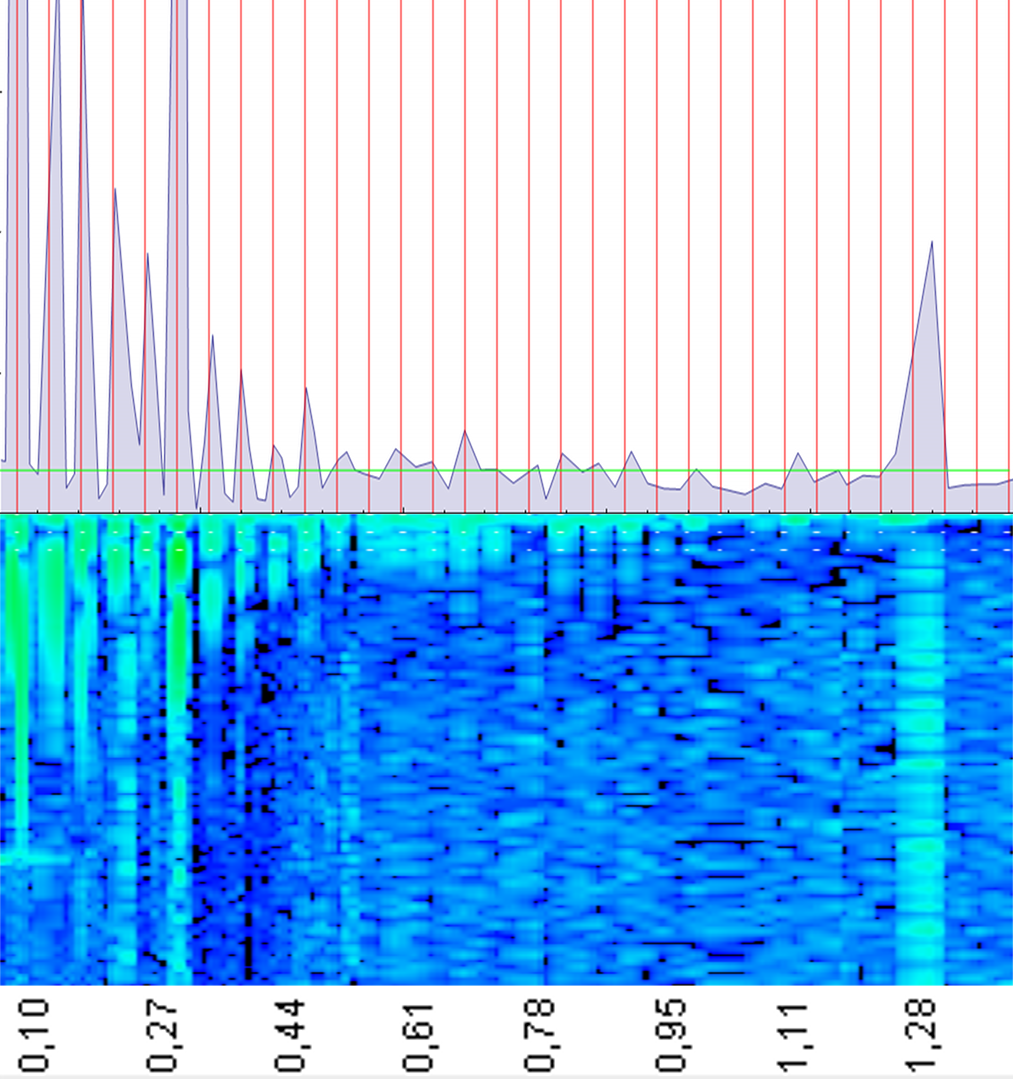
\includegraphics[width=140mm]{images/column_sums_orbit_3974_000.png}
	\caption{The column sums of a part of ionogram. The ionogram below is displayed along the sounding frequency scale in MHz. The top part shows the column sums at the frequencies from ionogram. The red lines represent the harmonics of the manually measured repetition period. They very closely correspond to the peaks in column sums. The green horizontal line denotes the mean value of the sums.}
	\label{fig:colSums}
\end{figure}

\subsection{Simplification in the case of ionograms}
The general definition assumes we are looking for point-like structures (given by 2~coordinates) and thus requires computing the histogram along at least two axes. From two histograms both 2D coordinates can be determined, but often there are ambiguities in the solution (for features overlapping in the direction perpendicular to an axis) \citep[chap.~13]{Davies2004}. The removal of such ambiguities is not trivial. 

Fortunately, in the ionogram case, only one axis is sufficient for every feature, since we are not interested in the length of the echo lines. Having the one histogram, detection of its peaks is all that is needed. Not all peaks in the histogram correspond to a harmonics line, some lower of them can be caused by noise. We call the peaks from harmonic lines ``real peaks'' and the others ``false peaks''. Our methods try to minimize the influence of false peaks by weighing them.

\section{Implementation}
We implemented our feature detector using the lateral histograms technique on evenly sampled ionograms. It can be found on the attached CD in directory \texttt{programs/detector-summing}. See \nameref{sec:running} for information on how to run it. 

\subsection{Finding and filtering the peaks}
Due to the properties of both EPOH and ECH we can reduce the problem to working on the left half of ionograms. It may happen that some EPOHs stretch beyond the half, but in such cases there have to be lots of other harmonic lines in the left part (since the harmonics are the stronger the closer they are to the base frequency). As all ECHs start at the left border and usually are not very long, cutting the image in half is also possible.

As stated above, not all peaks in the histogram belong to the harmonic echoes. In order to find only the high peaks, we first filter out \n[\%]{50} of the row/column sums with the lowest values. We should be able to detect periods of length 2 bins (the original unevenly sampled frequency columns), which would give just the \n[\%]{50} threshold. As can be derived from \citep[p.~3]{Akalin2010}, detecting periods less than \n{2.5} bins is impractical in the time domain, which yields threshold of \n[\%]{60}. As echoes in the frequency domain have to be sparser (due to the quasi-logarithmic spacing and quantization to bins), we can use this threshold, too.

With the uninteresting values filtered out (by setting them to zero) we can proceed to finding the peaks. The algorithm is rather simple, it just treats as a peak every data point with both neighboring values lower or equal to it. Once it finds a peak it zeroes out both non-increasing sequences neighboring to it (to get rid of non-strict maxima). What remains are the highest local maxima of the histogram. A visualization of the steps is shown in Figure \ref{fig:colSumsFiltering}.

\begin{figure}
	\centering
	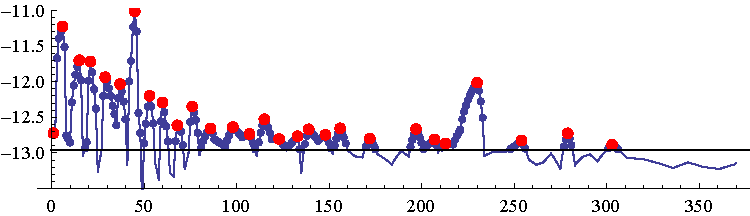
\includegraphics[width=140mm]{images/col_sums_peak_filtering.pdf}
	\caption{The steps to do when filtering the peaks within column sums in order to find the highest peaks. The blue lines are the original column sums. The blue dots are the column sums over the \mbox{\n{0.6}-quantile} represented by the black line. We seek for the peaks among these values. The peaks are marked with the larger red dots.}
	\label{fig:colSumsFiltering}
\end{figure}

\subsection{Using the peaks of row/column sums}
In an ideal case the set of peaks would contain all the harmonic lines positions and no more. In practice, noise and data inaccuracies introduce some false peaks. As a heuristic to tell if a peak comes from harmonic lines, we can look at its height. The echo lines are often long and have their values more than 10~times higher than the background around them. Both these facts contribute to greater values of the row/column sums. For EPOH, if there are some ECH lines or an IE in the image, they disappear in the peaks list. It is because they are perpendicular to the EPOH lines and so may fill up the space between EPOHs, but in the frequency domain, their contribution is relatively small in comparison with the contribution of the EPOH lines. Ground echoes are almost completely discarded by cutting the ionogram in half. Similarly, while detecting ECH lines, the EPOH lines should cause no trouble. However, an IE can cause problems because it usually adds a very high and broad peak to row sums. This is a caveat of using this method to detect ECHs. The only way to overcome this seems to be to narrow down the examined portion of ionogram to a range about \n{0.1}--\n[MHz]{0.8} (where the IE usually does not occur). The drawback is the narrowing allows for more important effects of noise. So we rather examine the whole half of the ionogram with bearing in mind that if other algorithms discover an IE in the ionogram, the vPeriod is most malformed.

We should also be able to recognize when there are no data of interest in the ionogram. Using just row/column sums it would have been, however, more a statistical than algorithmic decision. We could say what levels of row/column sums mean no feature is present. Or we could try to measure the ``ruggedness'' of the histogram to tell if there are some peaks. But we chose to rather not do such estimates and instead allow false positive detections. Removal of the false positives can be done later by comparing to the results of other methods more suitable to tell that a feature is not present at all. 

So we have the peaks and their heights as heuristics (telling us the probability of them to come from a line of interest). Combining these, we are finally able to estimate the repeat frequency. The last remaining task is to find a method taking peak positions and their weights (corresponding to their heights; we always normalize the weights) and computing the most probable period. The following section lists our three implemented methods -- the periodogram method, sine wave least squares fitting method and period averaging.

\section{Period estimation}
A period estimation method has to count with the fact that there are some peaks missing and some of them are extra. It should hold that the extra peaks have relatively low weights. On the other hand, some ``regular'' peaks can also have low weights. Again, there is no absolute rule on the weights of the peaks.

\subsection{Periodograms}
\label{ssec:periodogram}
The first proposed method is determination of the period from periodograms. Periodograms are defined in \citep{Scargle1982} for time series data. We slightly modify this definition to fit our purposes. Treat our set of peaks as a random variable $X$ measured at pixels $t_i$ along the axis (pixels without a peak yield zeros, the other ones). The measured values are denoted $\lbrace X_i = X(t_i): i = 1, 2, \ldots, N_0 \rbrace$. In our case, $N_0$ is the number of pixels along the axis. 

Having all the peaks the same unit height, we can now try to search for a sine wave with unit amplitude that would cross all the peaks. As the heights of the peaks are equal to the amplitude, it is required that the wave crosses the peaks exactly at its local maxima. Since sine is a periodic function and reaches its maximum once a period, the period of repetition should be equal to the period to be found between peaks.

We first present a simple form of periodogram which is fundamental for understanding the principles behind periodograms. The periodogram of random variable $X$ at frequency $\omega$ is by \citep{Scargle1982} defined as: 
\begin{align}
P_X(\omega) &= \frac{1}{N_0} {\left| \sum\limits_{j=1}^{N_0} X(t_j) \exp(-\imath\omega t_j) \right|}^2 \\
&= \frac{1}{N_0} \left[ \left( \sum\limits_{j=1}^{N_0} X(t_j)\cos\omega t_j \right)^2 + \left(\sum\limits_{j=1}^{N_0} X(t_j)\sin\omega t_j  \right)^2 \right]
\label{eq:periodogramClassic}
\end{align}
The explanation of the meaning of this expression is ``that if X contains a sinusoidal component of frequency $\omega_0$, then at and near $\omega = \omega_0$ the factors $X(t)$ and $\exp(-\imath\omega t)$ are in phase and make a large contribution to the sums in equation \eqref{eq:periodogramClassic}. At other values of $\omega$ the terms in the sum are randomly positive and negative, and the resulting cancellation yields a small sum.'' \citep[p.~836]{Scargle1982} This means that there should be high distinctive peaks of $P_X$ near the $\omega$ values close to the frequency of the sinusoid. 

Another important fact is that it is sufficient to evaluate $P_X$ at a finite set of frequencies to get the correct one. This set is, according to \citep[p.~850]{Scargle1982}, as follows:
$$ \lbrace \omega_n = 2\pi n / N_0 \mid n = -N_0/2, \ldots, +N_0/2 \rbrace $$
The meaning of this set can be understood in this way: ``The fundamental frequency, $\omega_1 = 2\pi / N_0$, corresponds to a sine wave with frequency equal to the whole interval $N_0$. This is roughly the lowest frequency about which there is information in the data. The so-called Nyquist frequency, $\omega_N = \frac{1}{2}(2\pi/{\Delta t}) = \pi$ ($\Delta t = 1$ is the sampling of the interval) is roughly the highest frequency about which there is information, because $\Delta t$ is the shortest time interval spanned.'' \citep[pp.~850--851]{Scargle1982}.

Finally, we present a modified version of periodogram devised in \citep{Scargle1982}. The new definition has several benefits, but for us it is important that it is phase invariant (since we do not know the phase of the signal). The definition by \citep[p.~838]{Scargle1982} is the following:
\begin{align}
P_X(\omega) = \frac{1}{2} \left\lbrace \frac{\left[ \sum\limits_{j=1}^{N_0} X(t_j)\cos\omega (t_j - \tau) \right]^2}{\sum\limits_{j=1}^{N_0} \cos^2\omega (t_j - \tau)} + \frac{\left[\sum\limits_{j=1}^{N_0} X(t_j)\sin\omega (t_j - \tau) \right]^2}{\sum\limits_{j=1}^{N_0} \sin^2\omega (t_j - \tau)} \right\rbrace,
\label{eq:periodogramBetter}
\end{align} 
where $\tau$ can be computed from
\begin{align}
\tan(2\omega\tau) = \left. \left(\sum\limits_{j=0}^{N_0} \sin 2\omega t_j \right) \middle/ \left(\sum\limits_{j=0}^{N_0} \cos 2\omega t_j \right) \right.
\end{align} 
Summed up, $\tau$ is the term providing phase invariance. The form \eqref{eq:periodogramBetter} has also better statistical properties and can be used with uneven sampling (which we do not need)\citep[p.~849]{Scargle1982}.

Our implementation passes the list of peaks to the periodogram function $P_X$ and computes the periodogram for the $N_0$ frequencies $\omega_n$. Then it selects the highest peak and computes the period belonging to it. An example of the periodogram is shown in Figure \ref{fig:periodogram}. Unfortunately, we have not found out how to incorporate peak weights to the algorithm. We tried multiplying every peak with its weight. Compared to the unweighted case, the results were even worse. We also tried to select the best peak among the 10~highest peaks (according to the mean of the column sums corresponding to the peaks). But the assessment method is probably not so strong, so in most cases the total result remains unchanged. 

Our implementation can be found on the attached CD in folder \texttt{programs/detector-summing}. See \nameref{sec:running} for information on how to run it. The results of the detection can be found also on the CD in subfolders of folder \texttt{data/} -- they are files named \texttt{TRACE\_(orbit number)\_SUM\_PERIODOGRAM.XML}.

\begin{figure}
	\centering
	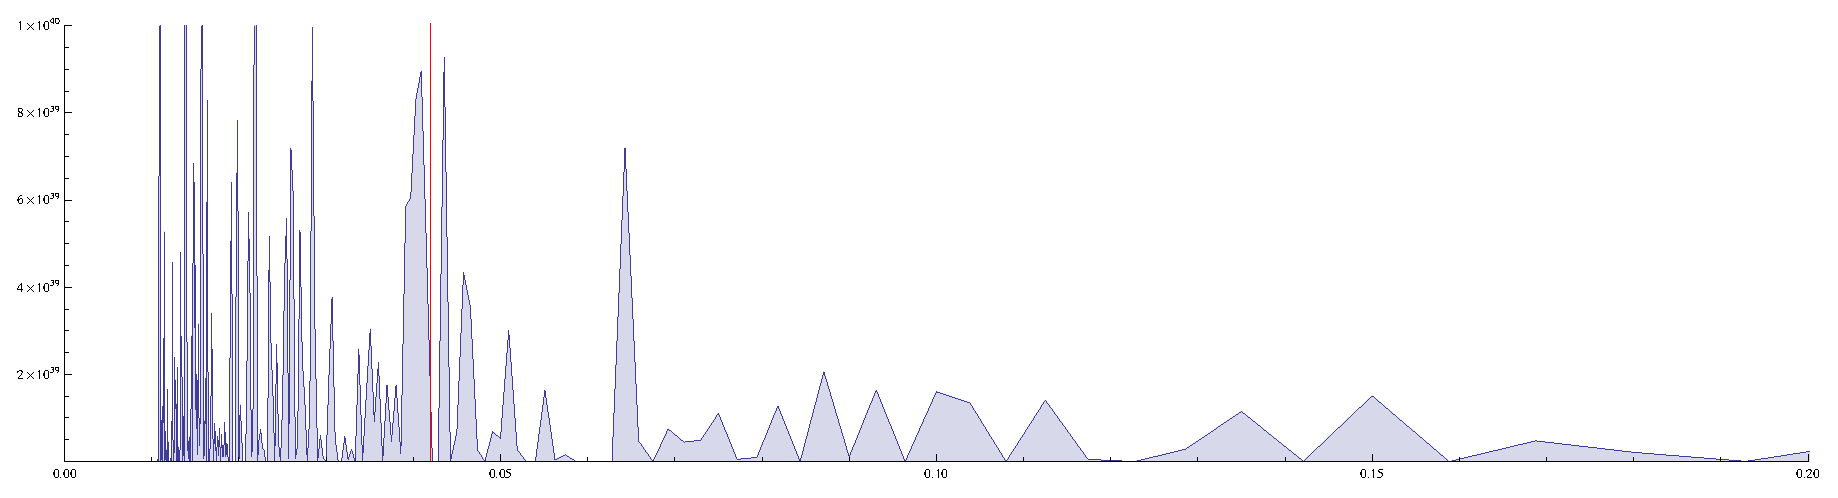
\includegraphics[width=140mm]{images/periodogram_from_normalized_peaks_orbit_3874_000.eps}
	\caption{The periodogram computed from the first ionogram in orbit 3874. The horizontal axis does not, however, show the frequency $\omega$ as is usual for periodograms, but it is already converted to correspond to the repetition period. The red vertical line is at the place of the manually measured repetiton frequency. It can be seen it tends to be near a large peak, but unfortunately at lower frequencies there are higher peaks that lead to incorrect results. The peaks in the left part are cropped at the top in order in interest of clarity.}
	\label{fig:periodogram}
\end{figure}
 
To assess the quality of the periodogram period estimation method, we perform two tests. In the first one we just measure the absolute difference between the estimated value and the manually acquired one; we denote it $E_A$. For simpler interpretation of the results we show the absolute error in ratio to the manually acquired value to get a percentage (for estimated period $p_e$ and manual period $p_m$ we compute~$E_A=|p_e-p_m|/p_m$). This is a nonuniform scaling, but it makes sense to require lower absolute errors for shorter periods.

We noticed that the estimated periods are often notable shorter than the target ones. After investigating the cause of this problem (which would render this method practically worthless) we found an explanation. Probably due to the (unweighted) false peaks the method tries to fit a sine wave which would go through all the real peaks as well as the false ones. This behavior makes the estimated periods be a ``1/integer'' fraction of the real period (eg. 1/2, 1/3, 1/4,~\ldots). This result looks interesting, because at least it allows us to considerably reduce the search space. Due to this property we also compute the second statistic $E_P$ (we call it the period corrected error) -- the error of the nearest integer multiple of the estimated period (that is $E_P=|round(p_m/p_e)\cdot p_e-p_m|/p_m$).

The results of these tests are shown in Figure \ref{fig:periodogram_errors}. As can be clearly seen, the absolute error $E_A$ with median~\n[\%]{68} shows the results to be completely useless. On the other hand, the period corrected error with median~\n[\%]{4.5} and \mbox{\n{0.75}-quartile}~\n[\%]{7.6} looks like a relatively good result. Average computation time (covering also the GE detection detailed in Section \ref{sec:ge_detection}) is about \n[s]{0.65} per ionogram of size \n{1012}$\times$\n[px]{506}.  

\begin{figure}
	\centering
	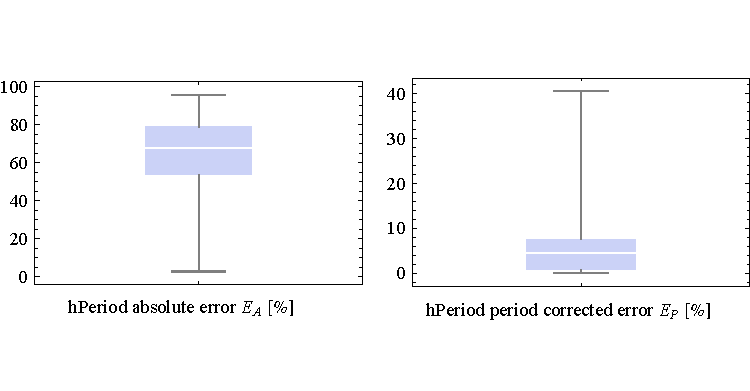
\includegraphics[width=140mm]{images/periodogram_errors.pdf}
	\caption{The errors of period estimation using the periodogram method. The tests were conducted on a set of ionograms from orbits 3836--4000. The left chart displays the absolute error $E_A$ with the \mbox{\n{0.25}-quartile}~=~\n[\%]{53}, median~=~\n[\%]{68} and the \mbox{\n{0.75}-quartile}~=~\n[\%]{79}. The right chart shows the period corrected error $E_P$ with the \mbox{\n{0.25}-quartile}~=~\n[\%]{0.8}, median~=~\n[\%]{4.5} and \mbox{\n{0.75}-quartile}~=~\n[\%]{7.6}.}
	\label{fig:periodogram_errors}
\end{figure}

To sum it up, the periodogram-based period estimation is not perfect for our task. On the other hand, its results can be utilized by other methods to scale down the search space. One more drawback is it only searches a fixed set of periods to try out.

\subsection{Sine wave least squares fitting}
The idea of fitting a sine wave to the peaks leads us to another algorithm. While the classical least squares fitting methods are suitable only for linear models to fit, there are also ways to do a similar fitting with nonlinear functions. One of these algorithms is the Levenberg-Marquardt algorithm introduced in \citep{Marquardt1963}.
 
We start with defining the model to fit, which is 
\begin{align}
E(y) = f(x; \beta_1, \ldots, \beta_k) = f(x, \boldsymbol\beta)
\end{align}
where $E(y)$ is the expected value. We simplify our case to a single variable, whereas \citep[p.~431]{Marquardt1963} describes the problem for any number of variables. Denote the peak values we have as $(Y_i, X_i), i = 1, \ldots N_0$. Then the least squares minimization problem is to find an assignment of $\beta$ that minimizes the error function 
\begin{align}
\Phi = \sum\limits_{i=1}^n[Y_i-\hat{Y}_i]^2 = \|\boldsymbol Y-\hat{\boldsymbol Y}\|^2,
\end{align}
where $\hat{Y}_i$ are the estimated values given by $E(y)$ \citep[p.~431]{Marquardt1963}.

For the algorithm we need the Jacobian matrix 
\begin{align}
J_j = \frac{\partial f(x)}{\partial b_j},\ j = 1, \ldots, k, 
\end{align}
where $b_j$ are the current estimates of $\beta_j$. We also need the vector
\begin{align}
\boldsymbol g = \left( (Y - f(x)) \frac{\partial f(x)}{\partial b_j}\right) = J^T(\boldsymbol Y - f(\boldsymbol b)),\ j = 1, \ldots, k.
\end{align}
Both these notions are defined in \citep[p.~433]{Marquardt1963}.

With these definitions we can describe the iterative Levenberg-Marquardt algorithm. We select the damping factor $0 < \lambda^{(1)} \leq 1$ (some guides on its selection are provided in \citep[p.~437]{Marquardt1963}). The initial parameter vector $\boldsymbol b^{(1)}$ has to be guessed and passed to the algorithm. In every iteration $r$ we solve the set of linear equations
\begin{align}
({J^{(r)}}^T J^{(r)} + \lambda^{(r)}I)\boldsymbol \delta^{(r)} = \boldsymbol g^{(r)}
\end{align}
for the difference $\boldsymbol \delta^{(r)}$ which is used in the next iteration to construct $\boldsymbol b^{(r+1)} = \boldsymbol b^{(r)} + \boldsymbol \delta^{(r)}$. Using $\boldsymbol b^{(r+1)}$ we can update $\Phi^{(r+1)}$. Then we choose new damping factor $\lambda^{(r+1)}$ and proceed to the next iteration (as described in \citep[pp.~437--428]{Marquardt1963}). The iterations are repeated until either a maximum number of iterations is exceeded, if $\Phi$ converges to~0 or if we encounter a local minimum of $\Phi$. 

With a good initial guess, the algorithm converges to the global minimum of~$\Phi$. However, the algorithm may often lodge in a local minimum of $\Phi$ instead. But by good strategy for choosing $\lambda$ it should be robust enough \citep[pp.~437--428]{Marquardt1963}.

In our experiments we used the implementation of the Levenberg-Marquardt (LM) algorithm provided by the library Apache Commons Math~3~\citep{Apache2013}. In addition to the above described algorithm, it also supports weighing the data (by simply incorporating the weights in the error function), which is exactly what we want. It also contains a procedure for getting the initial guess on parameters based on computation of several definite integrals and using linear least squares method. This method is described in the source code \citep{math3}.

In our approach we try to fit a sine wave with unit amplitude against the peaks with unit height. In order to magnify the effect of the weights, we also make square roots of all of them and then normalize them. This way more mid-value weights can affect the fitting, which usually helps, as we have observed.

Since we have both minimum and maximum constraints on the frequency, we have to tell these constraints to the LM algorithm. As the Apache Commons implementation does not support imposing constraints to the optimized variables, we simulate such constraints by returning $\pm1$ derivative in direction $\omega$ for values outside our boundaries. This seems to be sufficient.

Our implementation can be found on the attached CD in folder \texttt{programs/detector-summing}. See \nameref{sec:running} for information on how to run it. The results of the detection can be found also on the CD in subfolders of folder \texttt{data/} -- they are files named \texttt{TRACE\_(orbit number)\_SUM\_FITTING.XML}.

For quality assessment we use the same two metrics as for periodograms -- the absolute error $E_A$ and the period corrected error $E_P$, since the fitting algorithm also suffers from returning ``1/integer'' multiples of the real period. The reason is the same as for periodograms -- with some false peaks, a lower error can be achieved by doubling (or tripling, \ldots) the frequency.   

Final results of our tests are shown in Figure \ref{fig:fitting_errors}. Similarly to the periodograms, the absolute error $E_A$ with median~\n[\%]{49} renders the results to be worthless. In contrast to the periodograms, however, the period corrected error with median~\n[\%]{17} and \mbox{\n{0.75}-quartile}~\n[\%]{28} also cannot be treated as a good result. From these results it seems the curve fitting method is not a good solution to our problem. We think it may be due to the false peaks (although they should have small weights). Average computation time (covering also the GE detection detailed in Section \ref{sec:ge_detection}) is about \n[s]{3} per ionogram of size \n{1012}$\times$\n[px]{506}. It is really slow compared to the other methods, mainly due to the iterative base of this method.

\begin{figure}
	\centering
	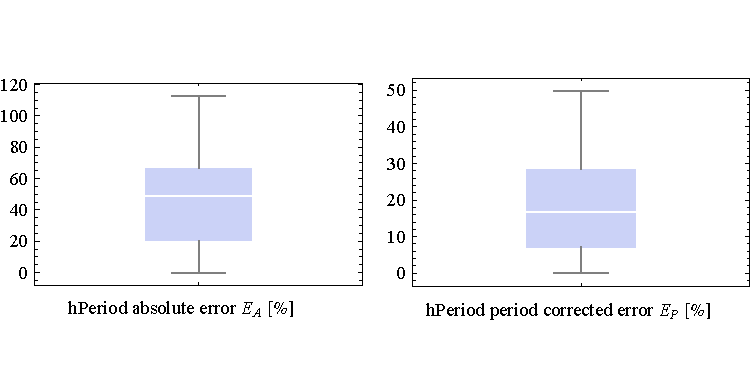
\includegraphics[width=140mm]{images/fitting_errors.pdf}
	\caption{The errors of period estimation using the sine wave fitting method. The tests were conducted on a set of ionograms from orbits 3836--4000. The left chart displays the absolute error $E_A$ with the \mbox{\n{0.25}-quartile}~=~\n[\%]{20.4}, median~=~\n[\%]{48.7} and the \mbox{\n{0.75}-quartile}~=~\n[\%]{66.7}. The right chart shows the period corrected error $E_P$ with the \mbox{\n{0.25}-quartile}~=~\n[\%]{7.1}, median~=~\n[\%]{16.7} and \mbox{\n{0.75}-quartile}~=~\n[\%]{28.4}.}
	\label{fig:fitting_errors}
\end{figure}

\subsection{Period averaging}
The last proposed way to determine the period from peaks and their weights is a method we call ``period averaging''. It utilizes a completely different approach than the previous methods.

On the input we again have the peaks with their weights. We first calculate the ``neighbor distances'' -- distances of the peaks being just one next to the other. This is the base for our approach. Each such distance gets a weight assigned that is equal to the weight of its right peak. In the ideal case without false peaks and with peaks for every harmonic line, simply computing a weighted average of these distances should give us the correct period. As we do not work with ideal data, we devised a method how to overcome the difficulties with false peaks and missing peaks for harmonic lines.

When we would just do a weighted average of the distances, a few missing harmonic lines could completely mislead the result (as well as the false peaks). E.g. we can take a period of 2~units. Then having 4~harmonics spaced correctly at the 2~units distance would give the correct period of 2~units. If these 4~lines were followed by 2~more lines spaced at 4~units (as if they were 4~lines and 2~of them disappeared, which is common in ionograms), then the average period would be $(4\cdot 2 + 2 \cdot 4)/6 = 8/3 \dot{=} 2.67$, which is an error of~\n[\%]{33.3}. This is unacceptable. Even the weighing does not help in this case beacause regular harmonic lines should have large weights (opposite to the false peaks which should have low weights and should not influence the result much).

We investigated the ionograms and we deduced that almost never more than a third of the harmonic lines is missing in the left half of ionograms (which we use in the rows/columns summing algorithm). So if we rule out (rounded off) \n[\%]{35} of the longest distances, we should not remove many correctly spaced peaks. On the other hand, all the long distances caused by missing harmonics should be eliminated. If there are no harmonics missing, we just eliminate some distances corresponding to the correctly spaced peaks, but since no harmonics are missing there must be several other correct distances left with high weights. As said earlier, false peaks should be smoothened out by their low weights.

So, with the resting \n[\%]{65} of distances, we re-normalize their weights. And with these weights we just evaluate the weighted arithmetic average of the distances and the harmonics period is found. 

Our implementation can be found on the attached CD in folder \texttt{programs/detector-summing}. See \nameref{sec:running} for information on how to run it. The results of the detection can be found also on the CD in subfolders of folder \texttt{data/} -- they are files named \texttt{TRACE\_(orbit number)\_SUM\_QUANTILE.XML}.

For quality evaluation we again use the absolute error $E_A$ and the period corrected error $E_P$. We expect the difference between $E_A$ and $E_P$ to be significantly lower than in the previous two methods (especially $E_A$ should be lower). That is since the period averaging should not tend the yield fractions of the real periods.   

The outcomes of our tests are shown in Figure \ref{fig:quantile_errors}. As expected, the absolute error $E_A$ is lower, with median~\n[\%]{23.5} being the best of the methods tested so far. What is a small disappointment for us is a relatively high $E_P$ -- with median~\n[\%]{9.73} and \mbox{\n{0.75}}-quartile~\n[\%]{22.5} it is not the best one. Average computation time (covering also the GE detection detailed in Section \ref{sec:ge_detection}) is about \n[s]{0.56} per ionogram of size \n{1012}$\times$\n[px]{506}.

\begin{figure}
	\centering
	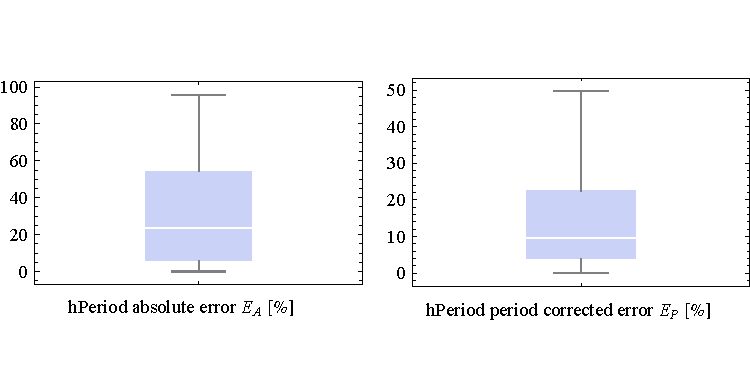
\includegraphics[width=140mm]{images/quantile_errors.pdf}
	\caption{The errors of period estimation using the period averaging method. The tests were conducted on a set of ionograms from orbits 3836--4000. The left chart displays the absolute error $E_A$ with the \mbox{\n{0.25}-quartile}~=~\n[\%]{5.7}, median~=~\n[\%]{23.5} and the \mbox{\n{0.75}-quartile}~=~\n[\%]{54}. The right chart shows the period corrected error $E_P$ with the \mbox{\n{0.25}-quartile}~=~\n[\%]{4}, median~=~\n[\%]{9.9} and \mbox{\n{0.75}-quartile}~=~\n[\%]{22.4}.}
	\label{fig:quantile_errors}
\end{figure}

\subsection{Combining the methods}
Taking into account the properties of the periodogram-based and average-based methods, there emerges a new, rather powerful and robust method for period estimation. As the periodogram-based method is good at determining the ``period corrected'' period (denote it $p_p$), the average-based method well estimates the ``magnitude'' of the period (denoted $p_a$). By magnitude we mean that the estimated period is not a fraction of the manually measured period $p_m$ (it is near this value, but still with a rather large error as mentioned in the previous section).

So we have the period $p_p$ about which we know that there exists an integer coefficient $c$ such that $c \cdot p_p \dot{=} p_m$. And we also know $p_a \dot{=} p_m$ but with a larger error. Se we propose to compute the integer $c$ as $\hat{c} = round(p_a/p_p)$ and then determine the period as $\hat{c} \cdot p_p$.

Because the periodogram-based method uses only a constant set of periods to try, we would be limited by these values, which could lead to unnecessary errors in the result. For this reason we weight both periods into the final result $\hat{p} = 0.5\cdot p_a + 0.5\cdot \hat{c}\cdot p_p$.  

Our implementation can be found on the attached CD in folder \texttt{programs/detector-summing}. See \nameref{sec:running} for information on how to run it. The results of the detection can be found also on the CD in subfolders of folder \texttt{data/} -- they are files named \texttt{TRACE\_(orbit number)\_SUM\_COMBINED.XML}.

The evaluation again consisted of expressing the absolute error $E_A$ and the period corrected error $E_P$. Our expectation is that the difference between $E_A$ and $E_P$ is insignificant, because there should remain almost no estimates needing the ``period correction''. Also $E_A$ should be the lowest observed so long.

The results of our tests are presented in Figure \ref{fig:combined_errors}. Following our expectations, the absolute error $E_A$ is low; with median~\n[\%]{14} it is the winner of this chapter. On the other side, \mbox{\n{0.75}}-quartile~\n[\%]{35} is not as good as we expected. The small difference between $E_A$ and $E_P$ is validated -- the median of $E_P$ is~\n[\%]{11.7} (which means that there stillremained some results influenced by period correction, which is interesting). Average computation time (covering also the GE detection detailed in Section \ref{sec:ge_detection}) is about \n[s]{0.60} per ionogram of size \n{1012}$\times$\n[px]{506}.

\begin{figure}
	\centering
	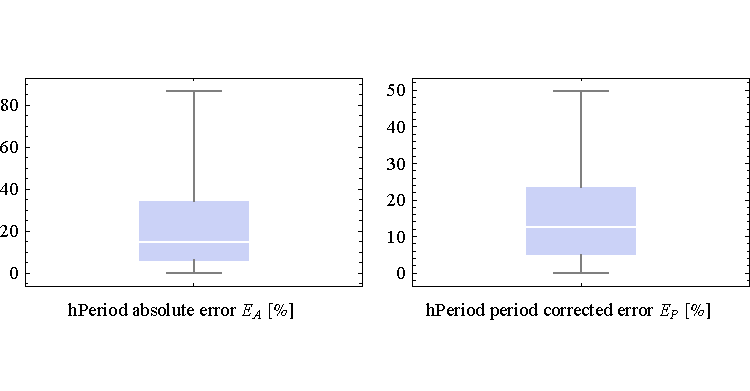
\includegraphics[width=140mm]{images/combined_errors.pdf}
	\caption{The errors of period estimation using the combined periodogram- and averaging-based method. The tests run on a set of ionograms from orbits 3836--4000. The left chart displays the absolute error $E_A$ with the \mbox{\n{0.25}-quartile}~=~\n[\%]{6.1}, median~=~\n[\%]{14.3} and the \mbox{\n{0.75}-quartile}~=~\n[\%]{34.6}. The right chart shows the period corrected error $E_P$ with the \mbox{\n{0.25}-quartile}~=~\n[\%]{5.2}, median~=~\n[\%]{11.7} and \mbox{\n{0.75}-quartile}~=~\n[\%]{22.9}.}
	\label{fig:combined_errors}
\end{figure}

\section{Vertical periods detection}
All the results presented above refer to the horizontal periods (EPOHs). Since we have no reference data for the vertical periods, we could not conduct such large statistical tests. So we just checked the estimated results with a small set of vertical periods extracted manually by ourselves. The result is not very good. The vertical periods use to be rather large (even a third of height of the ionogram and more), so there are not many echoes and the noise effects become significant. 

Also, the often stronger (and mainly longer) EPOHs behave as strong noise in this case -- they can even cause filtering out some vertical lines. As the EPOH-caused noise near the top part of the image (where EPOHs are the strongest) may reach rather high values, the real vertical peaks near bottom may fall under the \n[\%]{60} level used for peaks selection.

To conclude, we can say the detected vertical periods do not have significant relation to the real periods and their detection fails. As long as we do not have some larger set of verification data, solving this problem looks, however, impractical. 

\section{Ground echo detection}
\label{sec:ge_detection}
This last part of chapter about lateral histograms usage is dedicated to ground echo detection. With the knowledge of the current spacecraft height above surface (computed from the ephemeris data), we can predict the vertical position of ground echoes.

The first thing we do is decide whether a GE is present. This has two steps. The first is rather simple and only takes determining if the height above surface is less than the maximum detectable height. This boundary is limited by the \n[ms]{7.32} height of the vertical axis of ionograms. As radio waves spread approximately with the speed of light near Mars, the height corresponding to time delay $\Delta t$ is $c \cdot \Delta t / 2$ (the $/2$ for the signal path to surface and back, $c$ stands for the speed of light in vacuum). Supplying the maximum time delay to this equation, the maximum height at which a GE may appear is \n[km]{1098}.

The second decision step is based on row sums. We work only with the right half of the ionogram since this is where a GE may occur. We further divide the half of ionogram into two parts -- the rows near the possible GE occurrence (up to \n[px]{20} under than the possible occurrence for a ionogram sized \n{1012}$\times$\n[px]{506}), and other rows. Computing mean values of the electric field density in these two groups gives us a very good guiding principle for telling if a GE is present or not. If the mean in the group near GE is more than 2~times higher then in the rest, we tell a GE is present. The threshold value~2~was determined experimentally and seems to give good performance.

When we know we should look for a GE, we start at the right side of the ionogram and progress to its left (but we stop in the half). We begin on the row corresponding to the predicted GE occurrence. At every column we look at the values in the current row and \n[px]{10} under it and pick the highest of them. If this value is higher than the mean of rows near the possible GE as computed earlier, we consider it a part of the GE. If so, we also change the ``actual row'' to the row with the highest value before proceeding to the next column -- this makes the algorithm a tracking algorithm able to track even the cusp that may occur.

The results of the algorithm as described slightly differ from what we have defined as a result of GE detection. We defined the result should be the top edge of the GE and this algorithm instead finds the part with the highest values, which is commonly the centerline of the echo. We do not consider this a big problem because it may be processed further using a simple postprocessing, which, however, needs deeper information on the properties of the edge. As for the shape of the detected echo, it is nearly the same as the shape of the top edge of the GE.

As stated in Section \ref{ssec:results_spec}, we have not been provided with GE referential data. So the only assessment method available is visual comparison of a small set of detection results. As far as we can say, we have not found any ground echo with even a little bad shape, all the inspected ones precisely copied the shape of the ground echo. An example of a detected ground echo is given in Figure \ref{fig:ground_echo_detected}. We have also found no false negative detections (false positives may occur, though it is not frequent).

\begin{figure}
	\centering
	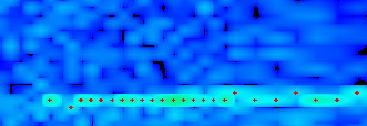
\includegraphics[width=140mm]{images/ground_echo_detected.png}
	\caption{An example of detected ground echo (the red dots). A cut of frame nr.~46~from orbit~3874.}
	\label{fig:ground_echo_detected}
\end{figure}

\section{Summary of lateral histogram methods}
We have presented a single method using the lateral histogram approach. This method may utilize one of the four proposed period estimation methods, of which the best is the combined method. As its error of estimation is about \n[\%]{14} we cannot say it is a perfect method (since manual tagging reaches a \n[\%]{1} error level), but it is definitely not worthless. All methods but sine wave fitting can be said to be relatively fast, with computation times about \n[s]{0.6} per ionogram. An example comparison of the detected periods is given in Figure \ref{fig:sums_comparison}.

We have also stated the the detection of the vertical period is a serious problem for this method. It needs further investigation to discover some really helpful noise-reducing techniques.

At last we have presented a very good way of determining the ground echoes in ionograms. It seems reliable as well as precise. We consider this as a good enough method for the precise measurements, although its detection error could not be validated due to the lack of reference data.

\begin{figure}
	\centering
	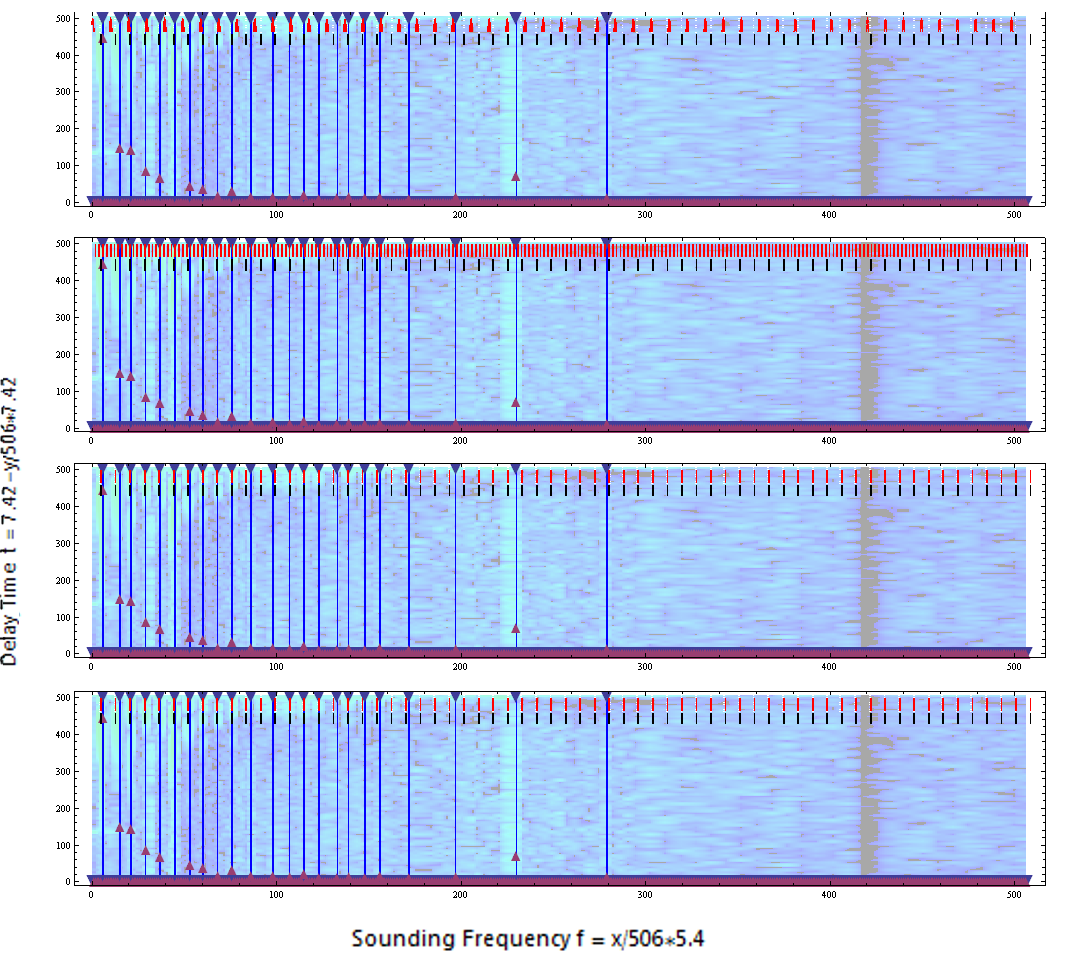
\includegraphics[width=140mm]{images/detected_period_fitting_periodogram_quantile_orbit_3874_000.png}
	\caption{A comparison of periods detected by the presented methods. Red ticks are the detected period. Black ticks denote the manually acquired period. Blue triangles as well as the blue lines correspond to peaks detected in the column sums. Purple triangles (with the tip up) are at positions corresponding to peak weights (multiplied by two for better visibility). From the top: the periodogram method, sine wave fitting method, average period method and the combined method. The ionogram in background is frame 0 in orbit 3874. Axis labels are in pixels of the evenly sampled ionogram. }
	\label{fig:sums_comparison}
\end{figure}